Se implementó un modelo de clasificación con el propósito de predecir y comprender el comportamiento del usuario basándose en un conjunto de datos detallado y complejo.

\subsection{Preprocesamiento y Preparación de Datos}

Comenzamos con la importación de los datos desde un archivo CSV, seguida de un proceso de limpieza para asegurar la integridad de la información. En esta etapa, se filtraron registros específicos en la columna “método” y se descartaron aquellos casos donde la columna “canal” estaba vacía. Adicionalmente, las marcas temporales fueron convertidas al formato UTC para garantizar una estandarización completa a lo largo del conjunto de datos.

El preprocesamiento es un paso fundamental para asegurarse de que los datos estén limpios, relevantes y listos para el modelado. Durante esta fase, se eliminan o corrigen valores atípicos, se manejan valores faltantes y se asegura la consistencia de los datos. Se filtraron métodos específicos y se eliminaron registros donde el canal estaba vacío para mantener solo los datos que contribuyen significativamente al análisis. La conversión de marcas temporales a UTC garantiza que todas las fechas y horas estén en un marco de referencia uniforme, lo cual es crítico para análisis temporales y comparaciones de eventos a través de diferentes zonas horarias.

\subsection{Ordenamiento y Etiquetado}

Para preservar la secuencia de acciones de cada usuario, ordenamos el conjunto de datos cronológicamente por usuario y fecha de evento. Este ordenamiento cronológico es esencial para cualquier modelo de clasificación secuencial, ya que permite comprender y aprender de las transiciones entre diferentes acciones o estados de un usuario. Específicamente, agrupamos las acciones por la columna ‘rut\_cliente’ y, dentro de cada grupo, las ordenamos por ‘fecha\_evento’ para mantener la secuencia temporal de las actividades.

Tras el ordenamiento, procedimos con la generación de etiquetas para la supervisión del aprendizaje. Excluyendo la última acción de cada secuencia o sesión, etiquetamos cada acción con la que le seguía, utilizando el método .shift(-1) en el DataFrame agrupado. Este enfoque desplaza las acciones hacia arriba, alineando así cada acción con su sucesora inmediata. Las acciones que seguían se usaron como etiquetas para la acción precedente. Para las últimas acciones de las secuencias, donde no hay una acción siguiente, asignamos una etiqueta especial, como 'final\_del\_recorrido', para indicar el término de la sesión.

Este proceso es fundamental para el entrenamiento de modelos de aprendizaje supervisado, especialmente para modelos secuenciales como las redes neuronales recurrentes (RNN) o las de memoria a corto y largo plazo (LSTM). Proporciona al modelo los 'objetivos' que necesita predecir, basándose en el contexto de las acciones previas. Al concluir este paso, cada acción en el conjunto de datos se asocia con una etiqueta que denota la acción inmediata futura, creando un conjunto de datos preparado para entrenar un modelo predictivo capaz de anticipar el comportamiento futuro del usuario a partir de su historial de interacciones.

\subsection{Identificación de Sesiones}

Para comprender mejor las interacciones de los usuarios con el sistema, segmentamos el flujo continuo de datos en sesiones discretas. Una sesión se define como una serie de eventos consecutivos realizados por un usuario, delimitada por períodos de inactividad que no superan un umbral de tiempo específico.

\textbf{Cálculo de Diferencias de Tiempo:} Iniciamos el proceso calculando el intervalo de tiempo entre eventos sucesivos para cada usuario. Esto se logró aplicando el método .diff() a la columna de marcas temporales, previamente ordenada por usuario y fecha de evento. El resultado de esta operación es una nueva columna que representa el tiempo transcurrido entre cada acción y la siguiente.

\textbf{Definición de un Umbral de Tiempo:} Establecimos un umbral temporal para identificar nuevas sesiones. Este umbral fue definido basándonos en el patrón de uso característico del sitio web, considerando que un lapso de más de 30 minutos sin actividad sugiere el fin de una sesión.

\textbf{Identificación de Nuevas Sesiones:} Comparando las diferencias de tiempo con nuestro umbral, pudimos identificar el inicio de nuevas sesiones. Un valor superior al umbral en la columna de diferencias de tiempo indica que la acción correspondiente es el comienzo de una nueva sesión.

\textbf{Asignación de Identificadores de Sesión:} Para marcar estas nuevas sesiones de manera clara, transformamos los valores booleanos resultantes de la comparación con el umbral en un identificador numérico acumulativo. Cada vez que se detecta una nueva sesión, este identificador se incrementa gracias al método .cumsum(), asignando así un número único a cada sesión para cada usuario.

El código utilizado para este proceso es el siguiente:

\begin{figure}[H]
    \begin{minipage}[t]{0.9\textwidth}
        \caption{Código indentificación de sesiones}
        \label{identificación_sesiones}        
    \end{minipage}

    \vspace{10pt}

    \begin{minipage}[b]{1\textwidth}
        \centering
        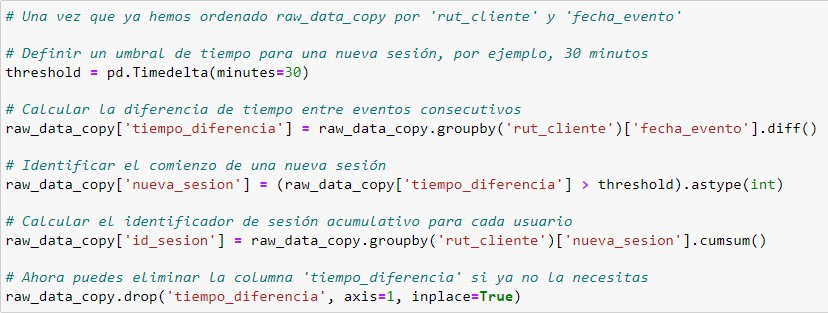
\includegraphics[width=\textwidth]{img/Código identificación sesiones.jpg}        
    \end{minipage}

    \begin{minipage}[t]{0.9\textwidth}
        Fuente: Elaboración propia.
    \end{minipage}
\end{figure}

Este método nos permitió estructurar el conjunto de datos de manera que refleja con precisión los períodos de interacción activa de los usuarios con el sistema, proporcionando una base sólida para el análisis y la modelación predictiva de su comportamiento futuro.

\subsection{Codificación de Categorías}

En el aprendizaje automático, es común encontrarse con datos categóricos, es decir, información que no está representada numéricamente, como los nombres de los métodos y canales en nuestro conjunto de datos. Para que estos datos puedan ser procesados por un modelo de clasificación, es necesario convertir estas categorías textuales en un formato numérico que el modelo pueda entender y manejar eficientemente. Este proceso se conoce como codificación de categorías y se llevó a cabo de la siguiente manera:

\textbf{Mapeo de Categorías a Números:}

\begin{itemize}
    \item Se crearon dos diccionarios: uno para \textbf{métodos} y otro para \textbf{canales}.
    \item Cada diccionario mapea una categoría textual única a un número entero único.
    \item Por ejemplo, el método \textbf{`login()`} podría mapearse al número 1, \textbf{`getAccounts()`} al número 2, y así sucesivamente.
\end{itemize}

\textbf{Mapeo de Categorías a Números:}

\begin{itemize}
    \item Utilizamos estos diccionarios para transformar todas las instancias de métodos y canales en nuestro DataFrame. Cada método y canal en el conjunto de datos fue reemplazado por su valor numérico correspondiente según los diccionarios de mapeo.
\end{itemize}

\textbf{Beneficios de la Codificación:}

\begin{itemize}
    \item Esta transformación es crucial porque los modelos de aprendizaje automático funcionan mejor con variables numéricas, las cuales pueden ser sujetas a operaciones matemáticas y estadísticas durante el entrenamiento del modelo.
    \item Además, la codificación permite el uso de algoritmos de incrustación (embedding) que pueden capturar y representar más información sobre las categorías en dimensiones más ricas que un simple número entero.
\end{itemize}

El código para implementar la codificación de categorías es el siguiente:

\begin{figure}[H]
    \begin{minipage}[t]{0.9\textwidth}
        \caption{Código codificación de categorías}
        \label{codificación_categorias}        
    \end{minipage}

    \vspace{10pt}

    \begin{minipage}[b]{1\textwidth}
        \centering
        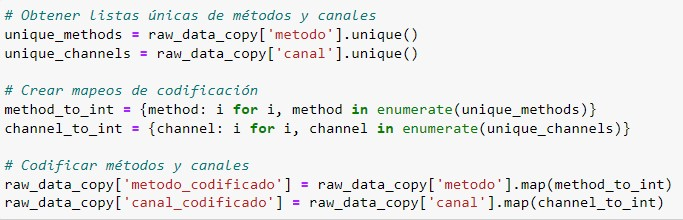
\includegraphics[width=\textwidth]{img/Código codificación categorias.jpg}        
    \end{minipage}

    \begin{minipage}[t]{0.9\textwidth}
        Fuente: Elaboración propia.
    \end{minipage}
\end{figure}

Esta etapa de codificación de categorías es un paso preparatorio esencial antes de alimentar los datos a nuestro modelo de clasificación secuencial. Permite que el modelo interprete adecuadamente los patrones en los métodos y canales como parte de la secuencia de acciones de un usuario y mejora la capacidad del modelo para hacer predicciones significativas sobre la próxima acción que el usuario podría tomar.

\subsection{Construcción de Secuencias}

La construcción de secuencias es un paso crucial en la preparación de datos para el modelado de series temporales o secuenciales, como es el caso de nuestro modelo de clasificación. Este proceso implica organizar los datos de tal manera que reflejen las secuencias naturales de interacciones de los usuarios. Veamos cómo se llevó a cabo:

\textbf{Agrupación de Eventos en Secuencias:}

\begin{itemize}
    \item Tras la codificación de los métodos y canales, cada acción del usuario está representada por un par de números codificados. El siguiente paso es agrupar estas acciones codificadas en secuencias que representan la trayectoria completa de la interacción del usuario dentro de una sesión.
    \item Cada secuencia se compone de pares de métodos y canales codificados y se crea para cada usuario y cada sesión identificada previamente. Esto se logra agrupando los datos por usuario y sesión y luego listando las acciones codificadas en orden cronológico.
\end{itemize}

\textbf{Preparación para el Modelo de Red Neuronal:}

\begin{itemize}
    \item Estas secuencias de números son lo que alimentará a la red neuronal. En el contexto de una LSTM o cualquier red neuronal recurrente (RNN), la secuencia permite al modelo reconocer patrones temporales y dependencias entre eventos consecutivos.
\end{itemize}

\textbf{Estructura de Datos de Secuencias:}

\begin{itemize}
    \item En términos de estructura de datos, las secuencias se manejan típicamente como listas de listas (o arrays de arrays) donde cada sublista representa una secuencia completa de un usuario.
\end{itemize}

El código para la construcción de secuencias es el siguiente:

\begin{figure}[H]
    \begin{minipage}[t]{0.9\textwidth}
        \caption{Código construcción de secuencias}
        \label{construcción_secuencias}        
    \end{minipage}

    \vspace{10pt}

    \begin{minipage}[b]{1\textwidth}
        \centering
        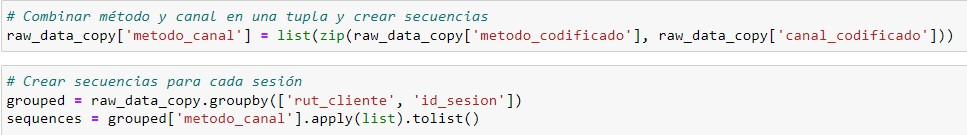
\includegraphics[width=\textwidth]{img/Código construcción de secuencias.jpg}        
    \end{minipage}

    \begin{minipage}[t]{0.9\textwidth}
        Fuente: Elaboración propia.
    \end{minipage}
\end{figure}

\textbf{Significado para el Modelado Predictivo:}

\begin{itemize}
    \item Estas secuencias son fundamentales para el modelado predictivo, ya que proporcionan el contexto completo necesario para que el modelo haga predicciones informadas. Por ejemplo, la secuencia de acciones anteriores de un usuario puede sugerir que la siguiente acción más probable podría ser 'cerrar sesión' después de una serie de consultas de información.
\end{itemize}

\textbf{Alineación con Objetivos de Predicción:}

\begin{itemize}
    \item Además, las secuencias están alineadas con las etiquetas que se generaron en el paso de etiquetado, donde cada acción excepto la última en una secuencia tiene una etiqueta correspondiente que indica la acción siguiente. Esto permite entrenar al modelo en la tarea de predecir la siguiente acción basándose en la secuencia de acciones anteriores.
\end{itemize}

La construcción de secuencias, por lo tanto, transforma un conjunto de eventos individuales en una serie de caminos estructurados que reflejan el comportamiento y las decisiones del usuario, lo que es esencial para entrenar un modelo que pueda anticipar las siguientes acciones en la ruta del usuario

\subsection{División de Datos}

La división de datos en conjuntos de entrenamiento y prueba es un paso fundamental en el desarrollo de modelos de aprendizaje automático. Este proceso es esencial para evaluar cómo el modelo generaliza datos no vistos anteriormente, es decir, su capacidad para hacer predicciones precisas en nuevas entradas fuera del conjunto de datos de entrenamiento. Veamos cómo se llevó a cabo este paso:

\textbf{Separación en Conjuntos de Entrenamiento y Prueba:}

\begin{itemize}
    \item El conjunto de datos completo se divide en dos partes: una para entrenar el modelo (conjunto de entrenamiento) y otra para probar su rendimiento (conjunto de prueba). Una práctica común es utilizar alrededor del 70-80\% de los datos para entrenamiento y el 20-30\% restante para pruebas.
\end{itemize}

\textbf{Aleatorización y Estratificación:}

\begin{itemize}
    \item La división debe hacerse de manera aleatoria para evitar sesgos en la selección de datos. Además, si el conjunto de datos es lo suficientemente grande y diverso, puede ser útil emplear una técnica llamada estratificación. Esto asegura que la proporción de las diferentes clases o categorías de respuesta se mantiene constante a través de ambos conjuntos.
\end{itemize}

\textbf{Importancia para la Validación del Modelo:}

\begin{itemize}
    \item La razón de separar los datos de esta manera es validar la capacidad del modelo para funcionar bien en condiciones reales. El conjunto de prueba actúa como un proxy para datos del mundo real que el modelo no ha visto durante su entrenamiento.
\end{itemize}

El código para dividir el conjunto corresponde al siguiente:

\begin{figure}[H]
    \begin{minipage}[t]{0.9\textwidth}
        \caption{Código dividir el conjunto}
        \label{dividir_conjunto}        
    \end{minipage}

    \vspace{10pt}

    \begin{minipage}[b]{1\textwidth}
        \centering
        \includegraphics[width=\textwidth]{img/Código dividir el conjunto de entrenamiento.jpg}        
    \end{minipage}

    \begin{minipage}[t]{0.9\textwidth}
        Fuente: Elaboración propia.
    \end{minipage}
\end{figure}

\textbf{Protección Contra el Sobreajuste:}

\begin{itemize}
    \item Al entrenar un modelo, siempre existe el riesgo de sobreajuste, donde el modelo se ajusta demasiado bien a los datos de entrenamiento, incluyendo el ruido o las peculiaridades específicas de ese conjunto de datos. La división de datos ayuda a detectar y mitigar el sobreajuste al proporcionar una medida más objetiva del rendimiento del modelo.
\end{itemize}

\textbf{Retroalimentación para la Iteración del Modelo:}

\begin{itemize}
    \item Los resultados en el conjunto de prueba proporcionan información valiosa que se puede utilizar para iterar y mejorar el modelo. Por ejemplo, si el modelo tiene un rendimiento significativamente peor en el conjunto de prueba en comparación con el conjunto de entrenamiento, esto es un indicador claro de sobreajuste.
\end{itemize}

\subsection{Construcción del Modelo}

La construcción del modelo es una etapa crucial en el proceso de aprendizaje automático, donde se define la arquitectura que se utilizará para aprender de los datos. En nuestro caso, se optó por un modelo de clasificación secuencial utilizando redes neuronales, específicamente una red neuronal recurrente (RNN) con Long Short-Term Memory (LSTM). A continuación, se detalla cómo se estructuró este modelo:

\textbf{Selección de la Arquitectura:} 
\begin{itemize}
    \item Elegimos una RNN con unidades LSTM debido a su eficacia en el manejo de datos secuenciales. Las LSTM son especialmente buenas para aprender dependencias de largo plazo en los datos, lo que las hace ideales para tareas como la predicción de la próxima acción de un usuario basada en su historial de acciones.
\end{itemize}

\textbf{Capa de Incrustación (Embedding):} 
\begin{itemize}
    \item El modelo comienza con una capa de incrustación. Esta capa transforma los índices de métodos y canales codificados en vectores densos de características. Esto permite que el modelo interprete mejor estas entradas categóricas y capture relaciones más complejas entre ellas.
\end{itemize}

\textbf{Capas LSTM:} 
\begin{itemize}
    \item Después de la capa de incrustación, agregamos una o más capas LSTM. Estas capas procesan los datos secuenciales, manteniendo un estado interno que refleja el contexto acumulado hasta el momento actual en la secuencia.
\end{itemize}

\textbf{Capa Densa de Salida:} 
\begin{itemize}
    \item La última capa del modelo es una capa densa con una unidad de salida por cada clase posible (en este caso, cada acción potencial siguiente). Esta capa utiliza la función de activación softmax para producir una distribución de probabilidad sobre las posibles acciones siguientes, lo que permite al modelo realizar una predicción.
\end{itemize}

\begin{figure}[H]
    \begin{minipage}[t]{0.9\textwidth}
        \caption{Construccion del modelo de clasificación}
        \label{parquitectura_clasificación}        
    \end{minipage}

    \vspace{10pt}

    \begin{minipage}[b]{1\textwidth}
        \centering
        \includegraphics[width=\textwidth]{img/Arquitectura modelo clasificación.jpg}        
    \end{minipage}

    \begin{minipage}[t]{0.9\textwidth}
        Fuente: Elaboración propia.
    \end{minipage}
\end{figure}

\subsection{Regularización y Compilación}

En esta etapa del desarrollo del modelo, nos enfocamos en dos aspectos clave: la regularización, para prevenir el sobreajuste, y la compilación, para definir cómo el modelo aprende durante el entrenamiento. Aquí te explico cómo abordamos estos dos puntos críticos:

\textbf{Regularización:} 
\begin{itemize}
    \item \textbf{Uso de Dropout:} Para prevenir el sobreajuste, implementamos capas de Dropout en la arquitectura del modelo. El Dropout es una técnica de regularización que aleatoriamente 'apaga' un porcentaje de neuronas durante cada iteración del entrenamiento. Esto evita que el modelo dependa demasiado de cualquier característica o camino específico, fomentando así que aprenda caminos redundantes y robustos para hacer predicciones. En nuestro modelo, se añadieron capas de Dropout después de las capas LSTM y posiblemente también después de las capas densas intermedias, con un ratio comúnmente entre 0.2 y 0.5.
\end{itemize}

\textbf{Compilación del Modelo:} 
\begin{itemize}
    \item \textbf{Elección del Optimizador:} Seleccionamos el optimizador 'Adam' para la compilación del modelo. Adam es ampliamente utilizado debido a su eficiencia en diferentes tipos de problemas de aprendizaje automático. Ajusta la tasa de aprendizaje de manera adaptativa, lo que lo hace adecuado para muchos escenarios sin necesidad de una afinación manual extensiva.
    \item \textbf{Función de Pérdida:} Utilizamos la 'categorical\_crossentropy' como nuestra función de pérdida, ya que estamos trabajando con un problema de clasificación multiclase. Esta función mide el rendimiento del modelo cuyas salidas son probabilidades; es efectiva para comparar la distribución de probabilidad predicha por el modelo con la distribución real representada por las etiquetas.
    \item \textbf{Métricas de Evaluación:} Elegimos 'accuracy' (precisión) como métrica para monitorear durante el entrenamiento. La precisión es una medida intuitiva y ampliamente utilizada que indica la proporción de predicciones correctas sobre el total de predicciones.
\end{itemize}

Código compilar modelo

\begin{figure}[H]
    \begin{minipage}[t]{0.9\textwidth}
        \caption{Construccion del compilador del modelo}
        \label{compilar_modelo}        
    \end{minipage}

    \vspace{10pt}

    \begin{minipage}[b]{1\textwidth}
        \centering
        \includegraphics[width=\textwidth]{img/Código compilar modelo.jpg}        
    \end{minipage}

    \begin{minipage}[t]{0.9\textwidth}
        Fuente: Elaboración propia.
    \end{minipage}
\end{figure}

\textbf{Balance entre Aprendizaje y Generalización:} La combinación de Dropout y una elección cuidadosa de la función de pérdida y el optimizador está destinada a lograr un equilibrio entre la capacidad del modelo para aprender eficientemente de los datos de entrenamiento (minimizando la pérdida) y su habilidad para generalizar bien a nuevos datos (maximizando la precisión en el conjunto de prueba).

\textbf{Preparación para el Entrenamiento:} Con el modelo ahora compilado, está listo para ser entrenado. La compilación efectiva asegura que el proceso de entrenamiento será eficiente y que el modelo tendrá una buena oportunidad de aprender patrones útiles de los datos sin memorizarlos, lo que es crucial para su rendimiento en escenarios del mundo real.


\subsection{Entrenamiento del Modelo}

El entrenamiento es la fase en la que el modelo de clasificación secuencial aprende de los datos. Durante este proceso, el modelo ajusta sus parámetros internos para minimizar el error en sus predicciones. A continuación, se detalla cómo se llevó a cabo el entrenamiento del modelo:


\textbf{Alimentación de Datos al Modelo:} El conjunto de datos de entrenamiento, que incluye tanto las secuencias de entrada (X\_train) como las etiquetas correspondientes (y\_train), se alimenta al modelo. El modelo aprende al ajustar sus pesos para predecir la etiqueta de cada secuencia de entrada lo más precisamente posible.

\textbf{Uso de Datos de Validación:} Paralelamente al entrenamiento, se utiliza un conjunto de validación (X\_test, y\_test) para evaluar el rendimiento del modelo. Esto proporciona una visión continua de cómo el modelo generaliza a datos no vistos, lo que es crucial para asegurarse de que el modelo no está sobreajustando los datos de entrenamiento.

\textbf{Configuración del Proceso de Entrenamiento:} El entrenamiento se lleva a cabo durante un número predefinido de iteraciones, conocidas como épocas. En cada época, el modelo procesa todo el conjunto de datos de entrenamiento.

\textbf{Monitoreo con EarlyStopping:} Para evitar el sobreajuste, implementamos un mecanismo llamado EarlyStopping. Este mecanismo monitorea la pérdida en el conjunto de validación y detiene el entrenamiento si esta pérdida no mejora después de un número determinado de épocas. Además, con la opción restore\_best\_weights, el modelo vuelve a los pesos que tenía en la época donde se logró la mejor pérdida de validación.

\textbf{Evaluación del Rendimiento:} Durante el entrenamiento, se monitorea la precisión y la pérdida tanto en los conjuntos de entrenamiento como de validación. Estas métricas son indicadores clave del rendimiento del modelo y ayudan a identificar si el modelo se está ajustando adecuadamente a los datos.

\begin{figure}[H]
    \begin{minipage}[t]{0.9\textwidth}
        \caption{Código para entrenar el modelo}
        \label{entrenar_modelo}        
    \end{minipage}

    \vspace{10pt}

    \begin{minipage}[b]{1\textwidth}
        \centering
        \includegraphics[width=\textwidth]{img/Código entrenar el modelo.jpg}        
    \end{minipage}

    \begin{minipage}[t]{0.9\textwidth}
        Fuente: Elaboración propia.
    \end{minipage}
\end{figure}


\subsection{Resultados del entrenamiento del modelo}

Después de completar el entrenamiento del modelo, evaluamos su rendimiento analizando las métricas de pérdida y precisión tanto en el conjunto de entrenamiento como en el de validación.

\begin{itemize}
    \item \textbf{Análisis de la Pérdida:} Los gráficos muestran que la pérdida de entrenamiento (Loss) y la pérdida de validación (Val\_Loss) disminuyen significativamente en las primeras épocas, lo que indica que el modelo está aprendiendo efectivamente de los datos. A medida que avanzan las épocas, ambas curvas de pérdida se estabilizan y convergen, lo que sugiere que el modelo ha alcanzado un punto donde realiza predicciones consistentes y fiables. La convergencia cercana de las dos líneas sugiere que el modelo no está sobreajustando, ya que la pérdida de validación no está aumentando ni divergiendo de la pérdida de entrenamiento.
    \item \textbf{Análisis de la Precisión:} En cuanto a la precisión, observamos que tanto la precisión de entrenamiento (Accuracy) como la precisión de validación (Val\_Accuracy) aumentan rápidamente y luego se estabilizan, manteniéndose muy cerca una de la otra. Esto indica un alto nivel de precisión en las predicciones del modelo y sugiere que el modelo generaliza bien a nuevos datos.
\end{itemize}

\begin{figure}[H]
    \begin{minipage}[t]{0.9\textwidth}
        \caption{Gráficos de análisis del modelo de clasificación}
        \label{gráfico_clasificación}        
    \end{minipage}

    \vspace{10pt}

    \begin{minipage}[b]{1\textwidth}
        \centering
        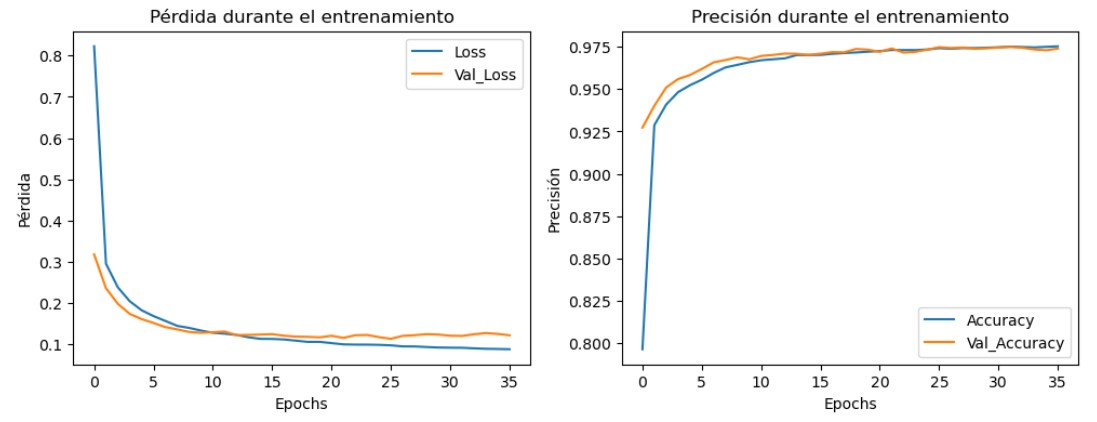
\includegraphics[width=\textwidth]{img/Gráfico modelo clasificación.jpg}        
    \end{minipage}

    \begin{minipage}[t]{0.9\textwidth}
        Fuente: Elaboración propia.
    \end{minipage}
\end{figure}

\subsection{Predicción del modelo}

Cuando usamos nuestro modelo de clasificación secuencial para hacer predicciones, se toma como entrada una secuencia de acciones anteriores realizadas por un usuario. Basándose en este historial, el modelo intenta predecir cuál será la próxima acción del usuario. Una característica clave de nuestro modelo es que no solo predice la siguiente acción más probable, sino que también estima la confianza en su predicción, expresada en términos de probabilidad.

Por ejemplo, si el historial de acciones del usuario sugiere que están en proceso de recabar información, y el modelo predice que la próxima acción será 'getDetails()', esta predicción vendrá acompañada de una probabilidad. Esta probabilidad, digamos un 95\%, representa la confianza del modelo en que 'getDetails()' será efectivamente la próxima acción del usuario. Esta medida de confianza es crucial para entender no solo qué espera el modelo que suceda a continuación, sino también cuán seguro está de esa expectativa.

En otro escenario, si un usuario ha estado interactuando con su cuenta, y el modelo predice que la próxima acción será 'getSSContributionsCertificate()', esta predicción podría tener una probabilidad asociada del 78.76\%. Esta cifra indica que, aunque el modelo inclina su predicción hacia 'getSSContributionsCertificate', hay una cierta incertidumbre, posiblemente debido a la variabilidad en el comportamiento del usuario o a patrones menos claros en las acciones previas.

Estos ejemplos ilustran cómo el modelo no solo toma decisiones binarias, sino que proporciona un contexto cuantitativo que puede ser invaluable para la toma de decisiones basada en datos, permitiendo a los sistemas o a los operadores humanos comprender mejor y reaccionar a las predicciones del modelo.